\documentclass[a4paper, 11pt]{article}
\usepackage[left=2cm,text={17cm, 24cm},top=3cm]{geometry}
\usepackage[czech]{babel}
\usepackage[utf8]{inputenc}
\usepackage[ruled, czech, linesnumbered, noline, longend]{algorithm2e}
\usepackage{times}
\usepackage{multirow}
\usepackage{graphics}
\usepackage{pdflscape}

\begin{document}
    \catcode`\-=12
    \begin{titlepage}
        \begin{center}
        	{\Huge\textsc{
				Vysoké učení technické v~Brně  \\
			}}
			{\huge\textsc{
				Fakulta informačních technologií \\
			}}
			\vspace{\stretch{0.382}}
			{\LARGE{Typografie a publikování \,--\, 3. projekt \\
			}}
			{\Huge{Tabulky a obrázky
			}}
			\vspace{\stretch{0.618}}
        \end{center}

        {\Large{\today \hfill Filip Pospíšil
        }}
    \end{titlepage}
    \section{Úvodní strana}
    Název práce umístěte do zlatéh ořezu a nezapomeňte uvést dnešní datum a vaše jméno a přijmení.
    \section{Tabulky}
    Pro sázení tabulek můžeme použít buď prostředí \verb|tabbing| nebo prostředí \verb|tabular|.
    \subsection{Prostředí \texttt{ tabbing}}
    Při použití \verb|tabbing| vypadá tabulka následovně:
    \begin{tabbing}
        Vodní melouny \quad \= \textbf{Cena} \quad  \= \textbf{Množství} \kill
        \textbf{Ovoce}  \> \textbf{Cena} \> \textbf{Množství} \\
        Jablka          \> 25,90         \> 3 kg\\
        Hrušky          \> 27,40         \> 2,5 kg\\
        Vodní melouny   \> 35,--         \> 1 kus\\
    \end{tabbing}
    Toto prostředí se dá také použít pro sázení algoritmů, ovšem vhodnější je použít prostředí \verb|algorithm| nebo \verb|algorithm2e| (viz sekce \ref{section:algoritmy}).
    \subsection{Prostředí \texttt{ tabular}}
    Další možností jak vytvořit tabulku, je použítí prostředí \verb|tabular|. Tabulky pak budou vypadat takto\footnote{Kdyby byl problém s \texttt{cline}, zkuste se pdoívat třeba sem:  http://www.abclinuxu.cz/tex/poradna/show/325037.}:
    \bigskip
     \begin{table}[h]
    		\centering
    		\begin{tabular}{|l|r|r|}
    			\hline
    							& \multicolumn{2}{c|}{\textbf{Cena}}	\\ \cline{2-3}
    			\textbf{Měna}	& \textbf{nákup}	& \textbf{prodej}	\\ \hline
    			EUR				& 25,615		    & 27,20				\\
    			GBP				& 29,899			& 31,80				\\
    			USD				& 22,571			& 25,51				\\ \hline
    		\end{tabular}
    		\caption{Tabulka kurzů k~dnešnímu dni}
    		\label{table:kurzy}
    \end{table}
    \bigskip
	\begin{table}[h]
		\centering
		\begin{tabular}[p]{|c|c|}
			\hline
			$ A $	    & $ {\neg}A $	\\ \hline
			\textbf{P}	& N				\\ \hline
			\textbf{O}	& O				\\ \hline
			\textbf{X}	& X				\\ \hline
			\textbf{N}	& P				\\ \hline
		\end{tabular}
		\begin{tabular}[p]{|c|c|c|c|c|c|}
			\hline
			\multicolumn{2}{|c|}{\multirow{2}{*}{$ A \wedge B $}} & \multicolumn{4}{c|}{$ B $}\\\cline{3-6}
			\multicolumn{2}{|c|}{} & \textbf{P} & \textbf{O} & \textbf{X}	& \textbf{N} \\ \hline
			\multirow{4}{*}{$ A $}	& \textbf{P} & P & O & X & N \\ \cline{2-6}
									& \textbf{O} & O & O & N & N \\ \cline{2-6}
									& \textbf{X} & X & N & X & N \\ \cline{2-6}
									& \textbf{N} & N & N & N & N \\ \hline
		\end{tabular}
		\begin{tabular}[p]{|c|c|c|c|c|c|}
			\hline
			\multicolumn{2}{|c|}{\multirow{2}{*}{$ A \vee B $}} & \multicolumn{4}{c |}{$ B $}
			\\ \cline{3-6}
			\multicolumn{2}{|c|}{} & \textbf{P} & \textbf{O} & \textbf{X}	& \textbf{N} \\ \hline
			\multirow{4}{*}{$ A $}	& \textbf{P} & P & P & P & P \\ \cline{2-6}
									& \textbf{O} & P & O & P & O \\ \cline{2-6}
									& \textbf{X} & P & P & X & X \\ \cline{2-6}
									& \textbf{N} & P & O & X & N \\ \hline
		\end{tabular}
		\begin{tabular}[p]{|c|c|c|c|c|c|}
			\hline
			\multicolumn{2}{|c|}{\multirow{2}{*}{$ A \rightarrow B $}} & \multicolumn{4}{c|}{$ B $}
			\\ \cline{3-6}
			\multicolumn{2}{|c|}{} & \textbf{P} & \textbf{O} & \textbf{X}	& \textbf{N} \\ \hline
			\multirow{4}{*}{$ A $}	& \textbf{P} & P & O & X & N \\ \cline{2-6}
									& \textbf{O} & P & O & P & O \\ \cline{2-6}
									& \textbf{X} & P & P & X & X \\ \cline{2-6}
									& \textbf{N} & P & P & P & P \\ \hline
		\end{tabular}
		\caption{
			Protože Kleeneho trojhodnotová logika už je \uv{zastaralá}, uvádíme si zde
			příklad čtyřhodnotové logiky
		}
		\label{table:logika}
    \end{table}
    \pagebreak
    \section{Algoritmy}
    \label{section:algoritmy}
    Pokud budeme chtít vysázet algoritmus, můžeme použít prostředí \verb|algorithm|\footnote{Pro nápovědu, jak zacháset s prostředím \texttt{algorithm}, můžete zkusit tuhle stránku:\\ http://ftp.cstug.cz/pub/tex/CTAN/macros/latex/contrib/algorithms/algorithms.pdf.} nebo \verb|algoritgm2e|\footnote{Pro \texttt{algorithm2e} zase tuhle: http://ftp.cstug.cz/pub/tex/CTAN/macros/latex/contrib/algorithm2e/doc/algorithm2e.pdf.}
    \IncMargin{1.5em}
	\begin{algorithm}
		\caption{\textsc{FastSLAM}}
		\label{algorithm:fastslam}
		\SetNlSty{}{}{:}
		\SetNlSkip{0.4em}
		\SetAlgoNlRelativeSize{-1}
		\SetInd{1em}{1em}
		\Indm\Indmm
		\KwIn{$(X_{t - 1},u_t,z_t)$}
		\KwOut{$X_t$}
		\Indp\Indpp
		\BlankLine
		$\overline{X_t}=X_t=0$ \\
		\For{$k=1\textrm{\emph{ to }}M$}{
			$x_t^{[k]}=\emph{sample\_motion\_model}(u_t,x_{t - 1}^{[k]})$\\
			$\omega_t^{[k]}=\emph{measurement\_model}(z_t,x_t^{[k]},m_{t - 1})$\\
			$m_t^{[k]}=updated\_occupancy\_grid(z_t,x_t^{[k]},m_{t - 1}^{[k]})$\\
			$\overline{X_t}=\overline{X_t}+\langle x_x^{[m]},\omega_t^{[m]}\rangle$\\}
		\For{$k = 1 \textrm{\emph{ to }}M$}{
			draw $i$ with probability $\approx\omega_t^{[i]}$\\
			add $\langle x_x^{[k]}, m_t^{[k]}\rangle\textrm{to}X_t$\\}
		\Return{$X_t$}
	\end{algorithm}
	\section{Obrázky}
    Do našich článků samozřejmě můžeme vkládat obrázky. Pokud je obrázkem fotografie, můžeme klidně použít bitmapový soubor. Pokud by to ale mělo být nějaké schéma nebo něco podobného, je dobrým zvykem takovýto obrázek vytvořit vektorově.
    \begin{figure}[h]
		\centering
		\scalebox{0.41}{
			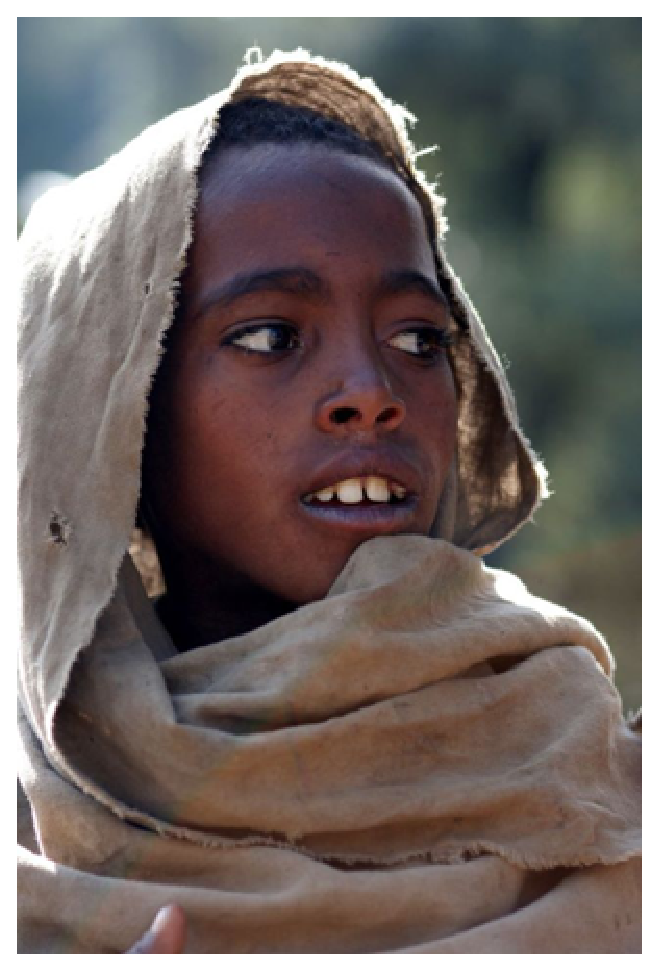
\includegraphics{obrazky/etiopan.eps}
			\reflectbox{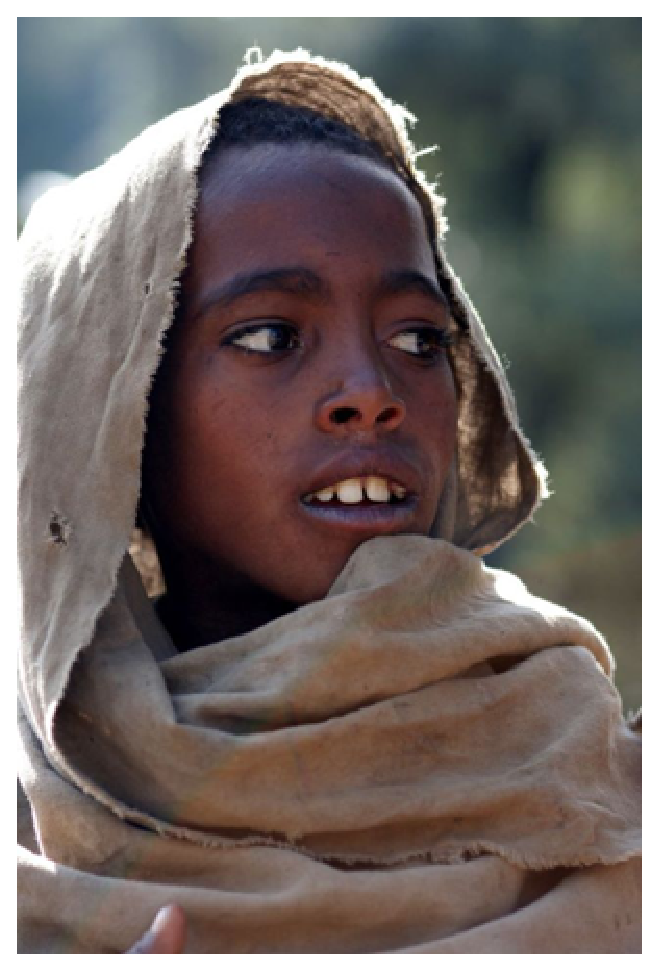
\includegraphics{obrazky/etiopan.eps}}
		}
		\caption{Malý Etiopánek a jeho bratříček}
		\label{figure:malyetiopan}
    \end{figure}
    \newpage
    \begin{figure}[h]
		\scalebox{0.41}{
\includegraphics{obrazky/oniisan.eps}}
		\centering
		\caption{Vektorový obrázek}
		\label{figure:vektorovy}
    \end{figure}
    \bigskip
    \noindent \dots a bitmapovým obrázkem

    \begin{figure}[h]
		\scalebox{0.62}{
\includegraphics{obrazky/oniisan2.eps}}
		\centering
		\caption{Bitmapový obrázek}
		\label{figure:bitmapovy}
    \end{figure}
    \bigskip
    \noindent se projeví například při zvětšení.

    Odkazy (nejen ty) na obárzky \ref{figure:malyetiopan}, \ref{figure:vektorovy} a \ref{figure:bitmapovy} a také na algoritmus \ref{algorithm:fastslam} jsou udělány pomocí křížových odkazů. Pak je ovšem potřeba zdrojový soubor přeložit dvakrát.

    Vektorové obrázky lze vytvořit i přímo v {\LaTeX}u, například pomocí prostředí \verb|picture|.

    \begin{landscape}
		\begin{figure}[h]
			\setlength{\unitlength}{1mm}
			\centering
            % variace na http://pospisil.redcoat.cz/fit/ity_3proj_predloha.jpg
			\begin{picture}(200, 160)
				\linethickness{1pt}
				\put(0, 0){\framebox(200, 150){}}

				\linethickness{1.8mm}
                \put(60,10){\line(1,0){115}}

                \linethickness{0.1mm}
                \put(25, 95){\line(1, 0){150}}
                \put(25, 60){\line(1, 0){150}}

                \linethickness{0.7mm}
                \put(60, 10){\line(0, 0){45}}
                \put(175, 10){\line(0, 0){90}}
                \put(25, 55){\line(1, 0){150}}
                \put(25, 100){\line(1, 0){150}}
                \put(25, 55){\line(0, 0){45}}

                \linethickness{0.4mm}
                \put(64, 10){\line(0, 0){42}}
                \put(64, 52){\line(1, 0){107}}
                \put(171, 10){\line(0, 0){42}}
                \put(99, 10){\line(0, 0){42}}
                \put(135, 10){\line(0, 0){42}}
                \put(40, 60){\line(0, 0){35}}
                \put(140, 60){\line(0, 0){35}}
                \put(40, 60){\line(1, 0){100}}
                \put(40, 95){\line(1, 0){100}}
                \put(65, 60){\line(0, 0){35}}
                \put(66, 60){\line(0, 0){35}}
                \put(67, 60){\line(0, 0){35}}
                \put(68, 60){\line(0, 0){35}}
                \put(69, 60){\line(0, 0){35}}
                \put(70, 60){\line(0, 0){35}}
                \put(71, 60){\line(0, 0){35}}
                \put(72, 60){\line(0, 0){35}}
                \put(73, 60){\line(0, 0){35}}
                \put(74, 60){\line(0, 0){35}}
                \put(75, 60){\line(0, 0){35}}
                \put(97, 60){\line(0, 0){13}}
                \put(119, 60){\line(0, 0){13}}
                \put(75, 60){\line(0, 0){13}}
                \put(75, 73){\line(1, 0){65}}


                \put(180, 130){\circle{17}}
			\end{picture}
			\caption{Vektorový obrázek moderního bydlení vhodného pro 21. století.}
		\end{figure}
\end{landscape}

\end{document}
